\documentclass[xetex,aspectratio=43]{beamer}

\usepackage{res/lections}

\preamble

\title{Общее устройство центрального процессора}

\begin{document}

    \titleslide

    \tocslide

\section{Блоки процессора}

\begin{frame}{Арифметико-логическое устройство}
    \defn{Арифметико-логическое устройство}{блок процессора, выполняющий арифметические и логические операции}
    \begin{itemize}
        \item В простейшем случае --- просто логическая схема
        \item Может использоваться для прикладных (например, вычисления, заданные программистом) и служебных (например, адресная арифметика)
        \item Имеет несколько входов для операндов и выход, на который \emph{мультиплексируются} выходы сумматора, мультипликатора и т.д.
    \end{itemize}
\end{frame}

\begin{frame}{Регистровый файл}
    \defn{Регистровый файл}{блок процессора, включающий набор регистров; внутренняя память процессора}
    \begin{outline}[itemize]
        \1 Арифметические регистры
            \2 Аккумулятор
            \2 Ещё несколько [десятков] регистров
        \1 Регистры состояний
            \2 Регистр флагов
        \1 Адресные регистры
            \2 Указатель вершины стека
            \2 Указатель на текущую инструкцию
            \2 Указатель на данные [часто несколько]
            \2 Вспомогательные (например, сегментные)
        \1 Служебные регистры
            \2 Хранение промежуточных значений, реализация протоколов (например, с ОЗУ) и т.д.
    \end{outline}
\end{frame}

\begin{frame}{Устройство чтения программы (блок выборки инструкций)}
    \defn{Устройство чтения программы}{блок процессора, выполняющий чтение очередных инструкций}
    \begin{outline}[itemize]
        \1 Читает из ОЗУ машинный код
            \2 Выполняет первичную интерпретацию машинного кода
    \end{outline}
    Для CISC-процессоров со сложным машинным кодом это не так-то просто!
\end{frame}

\begin{frame}{Управляющее устройство}
    \begin{outline}[itemize]
        \1 В зависимости от команды, выдаёт управляющие сигналы другим блокам процессора
            \2 Сигналы преимущественно управляют мультиплексорами, т.е. задают \emph{маршруты передачи данных между блоками процессора}
        \1 Если команда выполняется за много тактов (а обычно так и есть), выдаёт не один сигнал, а \emph{последовательность сигналов} разным блокам
    \end{outline}
\end{frame}

\section{Одно-, многотактный процессоры}

\begin{frame}{Однотактная схема}
    \begin{figure}
        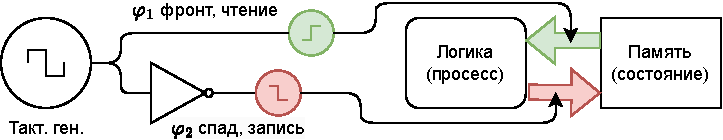
\includegraphics[width=\textwidth, page=1]{img/11.CPUS.drawio-crop.pdf}
    \end{figure}
    Вспоминаем:
    \begin{outline}[enumerate]
        \1 Синхронные и асинхронные вычисления, тактовый генератор, тактовые импульсы и тактовую сеть
        \1 Синхронизацию по фронту и спаду тактового импульса
        \1 Связку «master-slave»
        \1 Многофазные тактовые сигналы у старых процессоров
    \end{outline}
\end{frame}

\begin{frame}{Однотактный процессор}
    \begin{figure}
        \includegraphics[width=0.75\textwidth, page=2]{img/11.CPUS.drawio-crop.pdf}
    \end{figure}

    \begin{outline}[itemize]
        \1 В принципе, он даже может работать
            \2 Можно «нарисовать», например, несложный контроллер с такой архитектурой
        \1 Только гарвардский, т.к. нельзя одновременно обращаться и в одну память за кодом и данными
    \end{outline}
\end{frame}

\begin{frame}{Многотактный процессор}
    \vspace{-2mm}
    \begin{figure}
        \includegraphics[width=0.95\textwidth, page=3]{img/11.CPUS.drawio-crop.pdf}
    \end{figure}
    \vspace{-2mm}

    \begin{outline}[itemize]
        \1 Используются три фазы --- $\varphi_0, \varphi_1, \varphi_2$
            \2 Эти фазы может генерировать процессор внутри себя по сигналам обычного тактового генератора
        \1 Разные фазы выполняются разными блоками по очереди
            \2 $\frac{2}{3}$ времени блоки процессора простаивают!
    \end{outline}
\end{frame}

\section{Вычислительный конвейер}

\begin{frame}{Что такое конвейер?..}
    \alert{TODO}
\end{frame}


\begin{frame}{Вопросы и упражнения}
\begin{block}{Вопросы}
\begin{itemize}
\tightlist
\item
  Что такое
\end{itemize}
\end{block}

\begin{block}{Упражнения}
\begin{itemize}
\tightlist
\item
  Попробуйте
\end{itemize}
\end{block}
\end{frame}

\postamble

\end{document}
